\usetikzlibrary{decorations.pathmorphing}
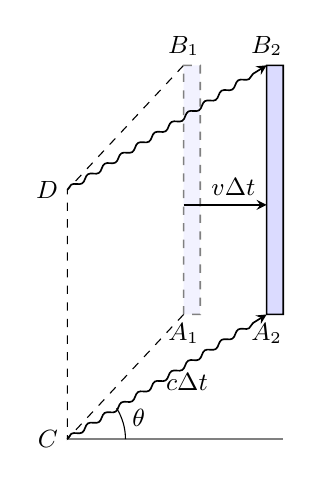
\begin{tikzpicture}[line width=0.2mm,scale=1.0545]\small
\tikzset{>=stealth}
\tikzset{snake it/.style={->,semithick,
decoration={snake,amplitude=.3mm,segment length=2.5mm,post length=0.9mm},decorate}}
\def\h{3}
\def\d{0.2}
\def\ww{1.4}
\def\w{1+\ww}
\def\p{1.5}
\def\r{0.7}
\coordinate[label=below:$A_1$] (A1) at (\ww,\p);
\coordinate[label=above:$B_1$] (B1) at (\ww,\p+\h);
\coordinate[label=below:$A_2$] (A2) at (\w,\p);
\coordinate[label=above:$B_2$] (B2) at (\w,\p+\h);
\coordinate[label=left:$C$] (C1) at (0,0);
\coordinate[label=left:$D$] (D) at (0,\h);
\draw[fill=blue!14](A2)--(B2)-- ++(\d,0)-- ++(0,-\h)--cycle;
\draw[gray,thin](C1)-- +(\w+\d,0);
\draw[dashed,gray,fill=blue!5](A1)-- (B1)-- ++(\d,0)-- ++(0,-\h)-- cycle;
\draw[dashed,line width=0.14mm](A1)--(C1)--(D)--(B1);
\draw[snake it](C1)--(A2) node[pos=0.6,below] {$c\Delta t$};
\draw[->,semithick](\ww,\p+0.44*\h)-- +(\w-\ww,0) node[pos=0.6,above] {$v\Delta t$};
\draw[snake it](D)--(B2);
\draw[thin](\r,0) arc (0:atan2(\p,\w):\r) node[midway,right,yshift=0.06cm] {$\theta$};
\draw[opacity=0](-0.40,-0.14)-- ++(0,5.06);
\end{tikzpicture}